\documentclass[20pt, a0paper, portrait, margin=0mm, innermargin=15mm,
               blockverticalspace=9mm, colspace=15mm, subcolspace=8mm]{tikzposter}
\usepackage[utf8]{inputenc}
\usepackage[T1]{fontenc}
\usepackage{amsmath}
\usepackage{booktabs}
\usepackage{graphicx}
\usepackage{qrcode}
\usepackage{enumitem}
\usepackage[table]{xcolor}
\usetikzlibrary{shapes.geometric, arrows.meta, positioning, fit, backgrounds, calc}

\definecolor{tecblue}{HTML}{0033A0}
\definecolor{tecdark}{HTML}{001A5C}
\definecolor{teclight}{HTML}{E8EEFA}
\definecolor{accent}{HTML}{E4572E}

\definecolorstyle{TecStyle}{}{
  \colorlet{colorOne}{tecblue}\colorlet{colorTwo}{tecdark}\colorlet{colorThree}{accent}}{
  \colorlet{backgroundcolor}{white}
  \colorlet{framecolor}{tecblue}
  \colorlet{titlefgcolor}{white}
  \colorlet{titlebgcolor}{tecblue}
  \colorlet{blocktitlebgcolor}{tecblue}
  \colorlet{blocktitlefgcolor}{white}
  \colorlet{blockbodybgcolor}{teclight}
  \colorlet{blockbodyfgcolor}{black}
  \colorlet{innerblocktitlebgcolor}{tecdark}
  \colorlet{innerblocktitlefgcolor}{white}
  \colorlet{notefillcolor}{teclight}
  \colorlet{notebordercolor}{tecblue}
  \colorlet{notefgcolor}{black}}
\usecolorstyle{TecStyle}
\usebackgroundstyle{Default}
\usetitlestyle{Filled}
\useblockstyle{Default}

\title{\parbox{0.9\linewidth}{\centering\bfseries Modelación de excedencias de ozono\\ en el área metropolitana de Monterrey}}
\author{Ricardo Salgado Benítez \;·\; Paola Mireles Ochoa \;·\; Aldo Javier Rodríguez Maytorena \;·\; Lenin Adolfo Caballero Colunga}
\institute{Equipo 6 — Aplicación de métodos multivariados en ciencia de datos (MA2003B), Grupo 201 \\
Tecnológico de Monterrey \;·\; Profesores: Dra. Blanca Rosa Ruíz Hernández, Dr. Jesús Jorge Armenta Seguroa}
\date{}

\usepackage{xspace}
\newcommand{\ppb}{\,ppb\xspace}
\newcommand{\tbox}[2]{\node[draw=tecblue, fill=white, rounded corners=6pt, line width=2pt, align=center,
  text width=#1, inner sep=10pt, font=\large] }

\makeatletter
\renewcommand{\TP@maketitle}{
  \centering
  \color{titlefgcolor}
  \begin{minipage}[c]{0.14\linewidth}
    \centering
\includegraphics[width=\linewidth]{sima.png}
  \end{minipage}\hfill
  \begin{minipage}[c]{0.70\linewidth}
    \centering
    {\bfseries \Huge \@title \par}
    \vspace*{1em}
    {\huge \@author \par}
    \vspace*{1em}
    {\LARGE \@institute \par}
  \end{minipage}\hfill
  \begin{minipage}[c]{0.14\linewidth}
    \centering
\includegraphics[width=\linewidth]{tec.png}
  \end{minipage}
}
\makeatother

\begin{document}
\maketitle
\raggedright\sloppy
\begin{columns}
%==================== COLUMNA 1 ====================
\column{0.5}

\block{Resumen}{
Se desarrolló un modelo de dos etapas para estimar, con un día de anticipación, la probabilidad de que el ozono (O$_3$) supere el límite horario de 90\ppb de la NOM-020-SSA1-2021 en cada una de las 15 estaciones del Sistema Integral de Monitoreo Ambiental (SIMA) del área metropolitana de Monterrey (AMM). Se usaron datos horarios de 2023 a julio de 2026, divididos cronológicamente en entrenamiento (2023--2024), validación (2025) y prueba (enero--julio 2026).

\vspace{4mm}
Como los días sobre la norma son pocos, la probabilidad se descompone en dos partes:

\vspace{2mm}
\begin{enumerate}
  \item Un modelo aditivo generalizado (GAM) binario, ajustado en conjunto para las 15 estaciones, que estima si el máximo de mañana superará un umbral auxiliar de 63\ppb a partir de la persistencia del ozono, la meteorología y el pronóstico de temperatura.
  \vspace{-5mm}
  \item Una distribución generalizada de Pareto (GPD), ajustada por picos sobre el umbral (POT), que extrapola hacia 90\ppb.
\end{enumerate}
\vspace{4mm}

En 2026 el modelo obtuvo un Brier Skill Score de 0.251 frente a la climatología y un AUC de 0.884; con el corte fijado en 2025 detectó 68.8\,\% de los días con exceso con 61.3\,\% de falsas alarmas. El riesgo sube con el ozono de hoy y con la temperatura pronosticada, y baja con el viento. Un análisis de dependencia de colas revela dependencia asintótica entre estaciones, ligada a su cercanía física y a la dispersión de contaminantes.
}

\block{Introducción}{
La contaminación atmosférica es un riesgo importante para la salud pública (enfermedades cardiovasculares y respiratorias). En el AMM, el crecimiento demográfico, la industria y una orografía rodeada de montañas favorecen la formación de esmog fotoquímico. El monitoreo del SIMA es retrospectivo: se requiere pasar de reaccionar a \textbf{prevenir} mediante alerta temprana.

\vspace{4mm}
\begin{itemize}[leftmargin=1.2em, itemsep=6pt]
  \item Los modelos físicos (WRF-Chem, CMAQ) son costosos, dependen de inventarios de emisiones desactualizados y subestiman picos locales.
  \item El aprendizaje automático que minimiza el error cuadrático suaviza las colas y falla en extremos (Wilson et al., 2022).
  \item La Teoría de Valores Extremos (POT--GPD) modela justamente las colas (Coles, 2001).
\end{itemize}

\vspace{4mm}
\textbf{Objetivo:} desarrollar, entrenar y validar un sistema de alerta temprana híbrido (GAM + GPD), interpretable y calibrado, que estime con 24 h de anticipación la probabilidad de excedencias de ozono en el AMM.
}

\block{Definición del problema}{
Predecir con 24 horas de anticipación la probabilidad de que el ozono supere \textbf{90\ppb} (límite horario de la NOM-020-SSA1-2021) en cada una de las 15 estaciones del SIMA, usando solo mediciones validadas, persistencia temporal y el pronóstico de temperatura de Open-Meteo.

\vspace{-2mm}
\begin{itemize}[leftmargin=1.2em, itemsep=6pt]
  \item \textbf{Desbalance severo:} solo 822 estación-días sobre la norma en entrenamiento, lo que dificulta a los clasificadores convencionales.
  \item \textbf{Costo de decidir:} una contingencia detiene actividades industriales y restringe la movilidad, por lo que se busca equilibrar detección de eventos y falsas alarmas.
\end{itemize}
}

\block{Metodología}{
\centering
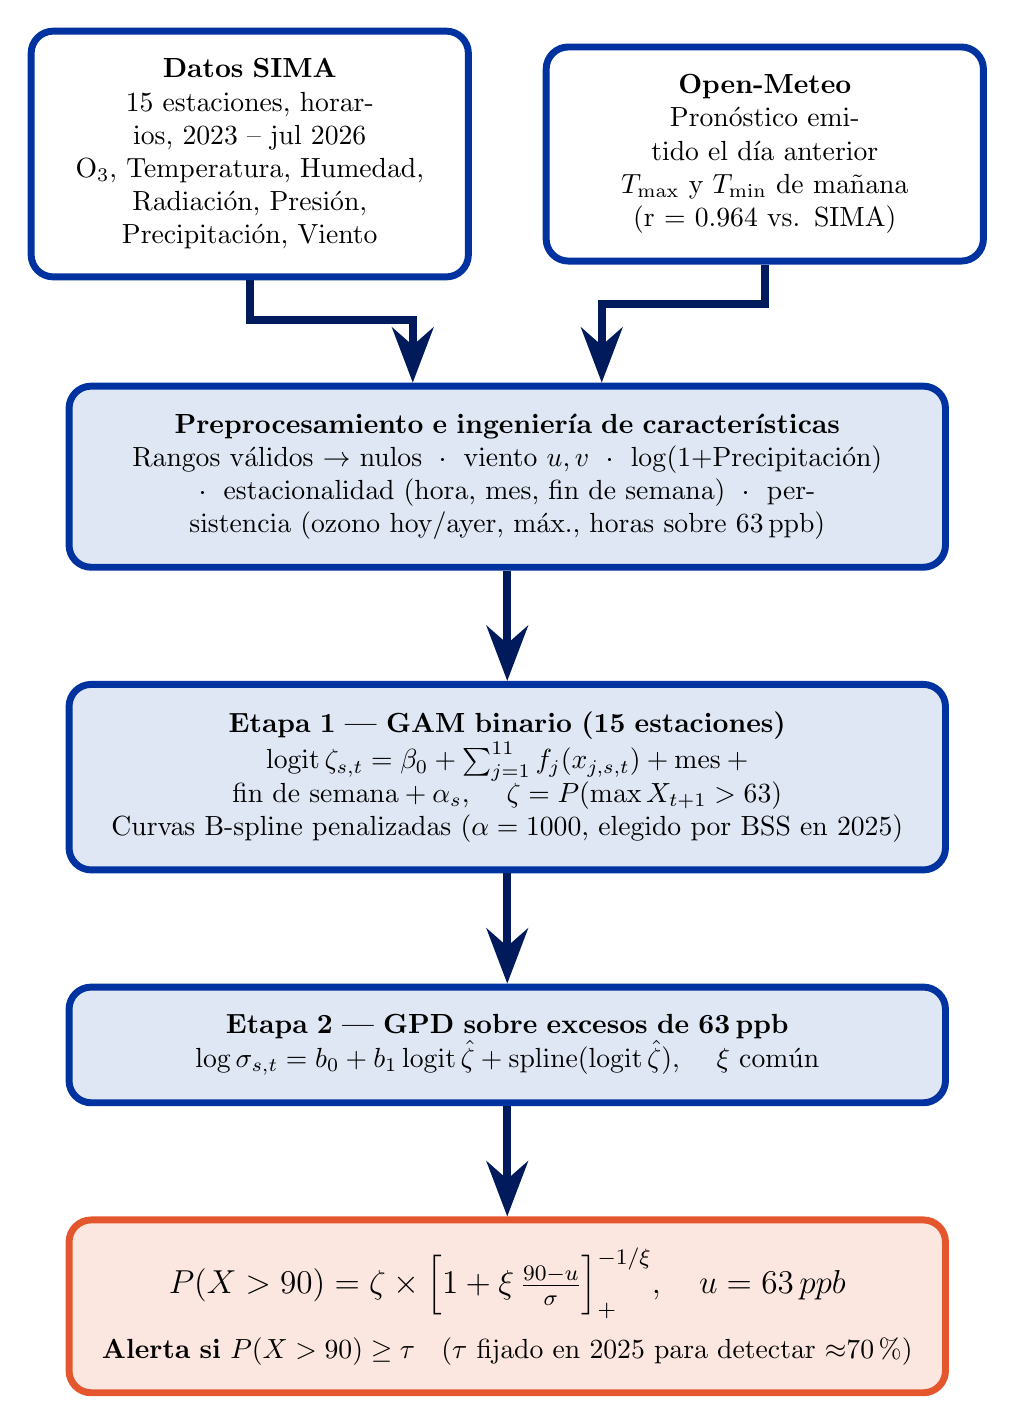
\begin{tikzpicture}[
  node distance=9mm, every node/.append style={},
  box/.style={draw=tecblue, fill=white, rounded corners=8pt, line width=2.5pt, align=center,
              text width=0.40\linewidth, inner sep=10pt, font=\normalsize},
  big/.style={box, fill=tecblue!12},
  arr/.style={-{Stealth[length=7mm]}, line width=3pt, color=tecdark}]
  \thinmuskip=3mu\medmuskip=4mu\thickmuskip=5mu
  \node[box] (d1) {\textbf{Datos SIMA}\\ 15 estaciones, horarios, 2023 -- jul 2026\\ O$_3$, Temperatura, Humedad, Radiación, Presión, Precipitación, Viento};
  \node[box, right=9mm of d1] (d2) {\textbf{Open-Meteo}\\ Pronóstico emitido el día anterior\\ $T_{\max}$ y $T_{\min}$ de mañana\\ (r = 0.964 vs. SIMA)};
  \node[big, anchor=north, text width=0.86\linewidth] (pre) at ($(d1.south)!0.5!(d2.south)-(0,14mm)$) {\textbf{Preprocesamiento e ingeniería de características}\\
    Rangos válidos $\to$ nulos \;·\; viento $u,v$ \;·\; $\log(1{+}\text{Precipitación})$ \;·\; estacionalidad (hora, mes, fin de semana) \;·\; persistencia (ozono hoy/ayer, máx., horas sobre 63\ppb)};
  \node[big, below=14mm of pre, text width=0.86\linewidth] (g1) {\textbf{Etapa 1 — GAM binario (15 estaciones)}\\
    $\mathrm{logit}\,\zeta_{s,t}=\beta_0+\sum_{j=1}^{11} f_j(x_{j,s,t})+\text{mes}+\text{fin de semana}+\alpha_s$, \quad $\zeta=P(\max X_{t+1}>63)$\\
    Curvas B-spline penalizadas ($\alpha=1000$, elegido por BSS en 2025)};
  \node[big, below=14mm of g1, text width=0.86\linewidth] (g2) {\textbf{Etapa 2 — GPD sobre excesos de 63\ppb}\\
    $\log\sigma_{s,t}=b_0+b_1\,\mathrm{logit}\,\hat\zeta+\text{spline}(\mathrm{logit}\,\hat\zeta)$, \quad $\xi$ común};
  \node[box, fill=accent!15, draw=accent, below=14mm of g2, text width=0.86\linewidth] (fin) {\large
    $\displaystyle P(X>90)=\zeta\times\Bigl[1+\xi\,\tfrac{90-u}{\sigma}\Bigr]_+^{-1/\xi},\quad u=63\ppb$\\[2mm]
    \normalsize \textbf{Alerta si $P(X>90)\ge\tau$} \; ($\tau$ fijado en 2025 para detectar $\approx$70\,\%)};
  \draw[arr] (d1.south) -- ++(0,-5mm) -| ($(pre.north)+(-12mm,0)$);
  \draw[arr] (d2.south) -- ++(0,-5mm) -| ($(pre.north)+(12mm,0)$);
  \draw[arr] (pre) -- (g1);
  \draw[arr] (g1) -- (g2);
  \draw[arr] (g2) -- (fin);
\end{tikzpicture}

\vspace{5mm}

\begin{tikzpicture}
  \def\W{0.86\linewidth}
  \fill[tecblue]    (0,0) rectangle (0.5*\W*0.5,1.2); \node[white] at (0.25*0.5*\W,0.6) {\bfseries Entrenamiento};
  \fill[tecblue!60] (0.5*\W*0.5,0) rectangle (0.5*\W*0.75,1.2); \node at (0.625*0.5*\W,0.6) {\bfseries Val.};
  \fill[accent!70]  (0.5*\W*0.75,0) rectangle (0.5*\W*1.0,1.2); \node at (0.875*0.5*\W,0.6) {\bfseries Prueba};
  \node[anchor=west, font=\normalsize] at (0.5*\W+0.3,0.6) {2023--24 \;|\; 2025 \;|\; ene--jul 2026 (partición cronológica)};
\end{tikzpicture}

\vspace{4mm}
\textbf{Técnicas multivariadas} 

\vspace{-2mm}
\begin{itemize}
  \item \textbf{Dependencia:} GAM / regresión logística binaria, GPD con escala no estacionaria.
  \item \textbf{Interdependencia:} componentes principales (ACP) del clima, dependencia de colas $\chi(q)$ y conglomerados jerárquicos con $1-\chi(0.95)$; prueba de Mantel.
\end{itemize}

}

%==================== COLUMNA 2 ====================
\column{0.5}

\block{Resultados}{
\innerblock{Efecto de cada variable sobre el riesgo (GAM)}{
\centering
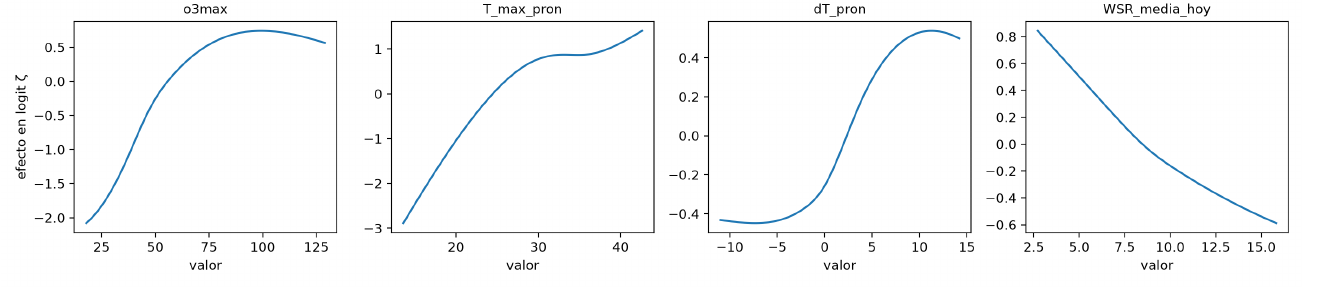
\includegraphics[width=0.94\linewidth]{fig4.png}\\[2mm]
\raggedright
El riesgo sube con el ozono máximo de hoy (se aplana cerca de 100\ppb) y con la temperatura máxima pronosticada; el viento lo reduce al dispersar el ozono. Cada unidad de $\mathrm{logit}\,\hat\zeta$ multiplica $\sigma$ por 1.46: los días de mayor riesgo también alcanzan mayores picos.
}

\innerblock{Comparación de modelos para $P(\text{máx. de mañana}>90\ \text{ppb})$}{
\centering
\normalsize
\renewcommand{\arraystretch}{1.35}
\begin{tabular}{lccccc}
\toprule
\textbf{Modelo} & \textbf{BSS 2025} & \textbf{BSS 2026} & \textbf{AUC 2026} & \textbf{Aciertos} & \textbf{Falsas al.}\\
\midrule
Climatología & 0 & 0 & 0.643 & 66.9\,\% & 84.1\,\%\\
Regresión logística + GPD & 0.202 & 0.252 & 0.890 & 70.3\,\% & 62.1\,\%\\
\rowcolor{tecblue!15}
\textbf{GAM + GPD (final)} & \textbf{0.224} & \textbf{0.251} & \textbf{0.884} & \textbf{68.8\,\%} & \textbf{61.3\,\%}\\
GAM con clima en ACP + GPD & 0.212 & 0.257 & 0.883 & 71.4\,\% & 60.7\,\%\\
Boosting directo & 0.214 & 0.236 & 0.880 & 70.8\,\% & 59.3\,\%\\
\bottomrule
\end{tabular}

\vspace{2mm}
{\footnotesize BSS: Brier skill score vs. climatología por estación. Aciertos y falsas alarmas en 2026 con corte fijado en 2025.}
}

\innerblock{Poder predictivo y calibración del GAM (2026)}{
\centering
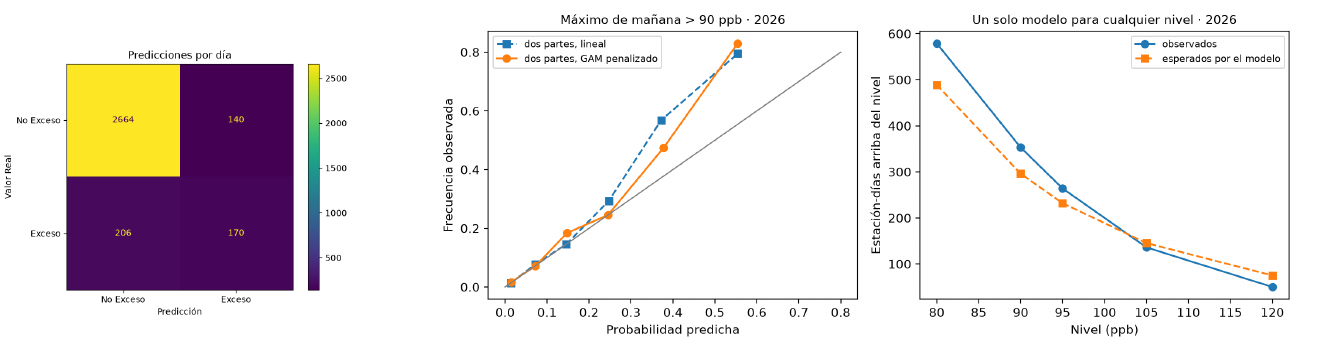
\includegraphics[width=0.92\linewidth]{fig7.png}\\[2mm]
\raggedright
Matriz de confusión (alerta si $p>0.30$): exactitud 89.1\,\%, precisión 54.8\,\%, sensibilidad 45.2\,\%. El GAM calibra bien hasta $\approx$0.25 y subestima por encima. La GPD estima correctamente la probabilidad de superar otros niveles (p. ej., 105\ppb: 136 observados vs. 145 esperados).
}

\innerblock{Dependencia de colas entre estaciones}{
\centering
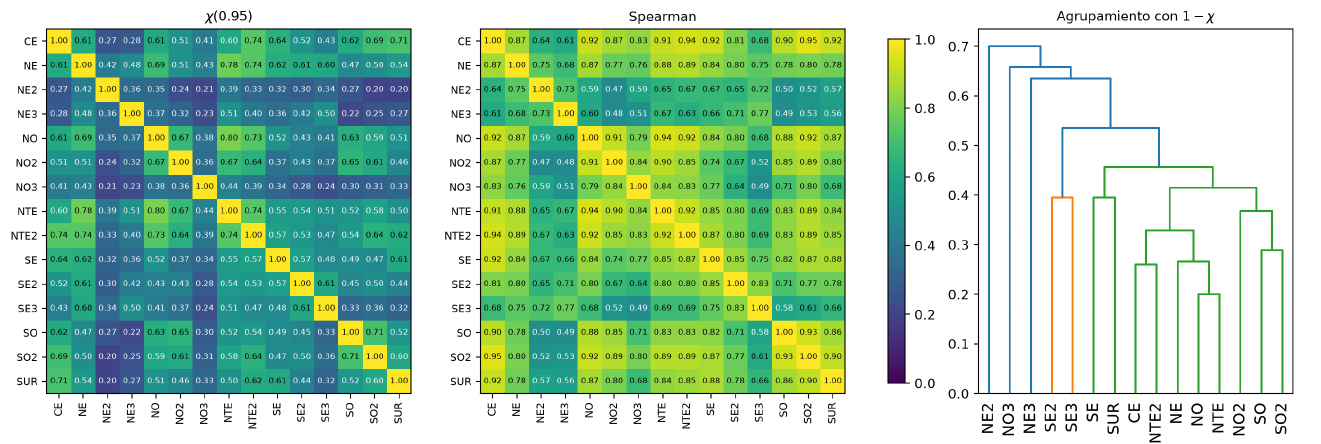
\includegraphics[width=0.90\linewidth]{fig5.png}\\[2mm]
\raggedright
Hay \textbf{dependencia asintótica}: cuando una estación vive un extremo, otras también (máx. $\chi(0.95)$: NO--NTE 0.80). Mantel entre distancia y $1-\chi$: $r=0.531$ ($p=0.0005$); la estacionalidad común no lo explica. Por ello, si una estación alerta, conviene alertar a todo el AMM: agrupando por día, la regresión logística + GPD alcanza AUC 0.904 y el GAM + GPD 0.883.
}

}

\block{Conclusiones}{
\begin{itemize}[leftmargin=1.2em, itemsep=8pt]
  \item El modelo GAM + GPD supera claramente a la climatología (BSS $\approx$0.25, AUC $\approx$0.88) y es \textbf{interpretable}: cumple los supuestos que la regresión logística incumple (linealidad en el logit).
  \item La regresión logística predice casi igual; la ventaja del GAM es la explicabilidad, no la precisión. Agrupando por día, la logística resulta mejor.
  \item Con $\approx$69\,\% de detección y $\approx$61\,\% de falsas alarmas, puede apoyar un sistema de alerta si se prioriza la sensibilidad; SIMA debe fijar el corte según el costo de cada tipo de error.
  \item \textbf{Limitaciones:} 2026 cubre solo siete meses, hay subestimación de los eventos más extremos y las métricas no tienen intervalos de incertidumbre.
  \item \textbf{Siguientes pasos:} definir la formulación (por estación o por AMM) con el socio formador e incorporar la dependencia espacial al modelo.
\end{itemize}
}

\block{Agradecimientos, código QR y contacto}{
\begin{minipage}{0.27\linewidth}
\centering
\qrcode[height=5.5cm]{https://REEMPLAZAR-CON-LIGA-DEL-VIDEO}\\[1mm]
{\small Video del proyecto}
\end{minipage}\hfill
\begin{minipage}{0.69\linewidth}
\normalsize
\textbf{Agradecimientos:} al SIMA de Nuevo León por los datos y el planteamiento del reto, y a la Dra. Blanca Rosa Ruíz Hernández y al Dr. Jesús Jorge Armenta Seguroa por su guía. Tecnológico de Monterrey.\\[3mm]
\textbf{Contacto:} \texttt{A01282489@tec.mx} \;·\; Código: \texttt{github.com/RicardoSalgadoB/MultiReto}
\end{minipage}
}

\end{columns}

\begin{columns}
\column{1}
\block{Referencias}{
\fontsize{17pt}{20pt}\selectfont\raggedright
Coles, S. (2001). \textit{An introduction to statistical modeling of extreme values}. Springer. \quad
Coles, S., Heffernan, J., \& Tawn, J. (1999). Dependence measures for extreme value analyses. \textit{Extremes, 2}(4), 339--365. \quad
García-Reynoso, J. A., \& Almanza, V. (2026). Advances in operational air quality forecasting for Mexico City. \textit{Atmósfera, 40}, 153--165. \quad
Gobierno del Estado de Nuevo León. (2025). \textit{Nuevo León anuncia histórica modernización del SIMA}. \quad
Gyarmati-Szabó, J., Bogachev, L. V., \& Chen, H. (2017). Nonstationary POT modelling of air pollution concentrations. \textit{Environmetrics, 28}(5), e2449. \quad
Jolliffe, I. T., \& Cadima, J. (2016). Principal component analysis: A review and recent developments. \textit{Phil. Trans. R. Soc. A, 374}(2065), 20150202. \quad
Mantel, N. (1967). The detection of disease clustering and a generalized regression approach. \textit{Cancer Research, 27}(2), 209--220. \quad
Ministerio del Medio Ambiente de Chile. (2021). \textit{Calidad del aire}. \quad
Secretaría de Salud. (2021). \textit{NOM-020-SSA1-2021, criterio para evaluar la calidad del aire ambiente con respecto al ozono (O$_3$)}. DOF, 28 de octubre de 2021. \quad
Sistema Integral de Monitoreo Ambiental. (2026). \textit{Diapositivas SIMA}. Tecnológico de Monterrey. \quad
Wilson, T., Tan, P.-N., \& Luo, L. (2022). DeepGPD: A deep learning approach for modeling geospatiotemporal extreme events. \textit{Proc. AAAI, 36}, 4245--4253. \quad
Wood, S. N. (2017). \textit{Generalized additive models: An introduction with R} (2.ª ed.). CRC Press. \quad
Zippenfenig, P. (2023). \textit{Open-Meteo.com weather API}. Zenodo. https://doi.org/10.5281/zenodo.7970649
}
\end{columns}
\end{document}